\documentclass[thesis.tex]{subfiles}
\begin{document}

\section{Datenblatt Body-Cam}

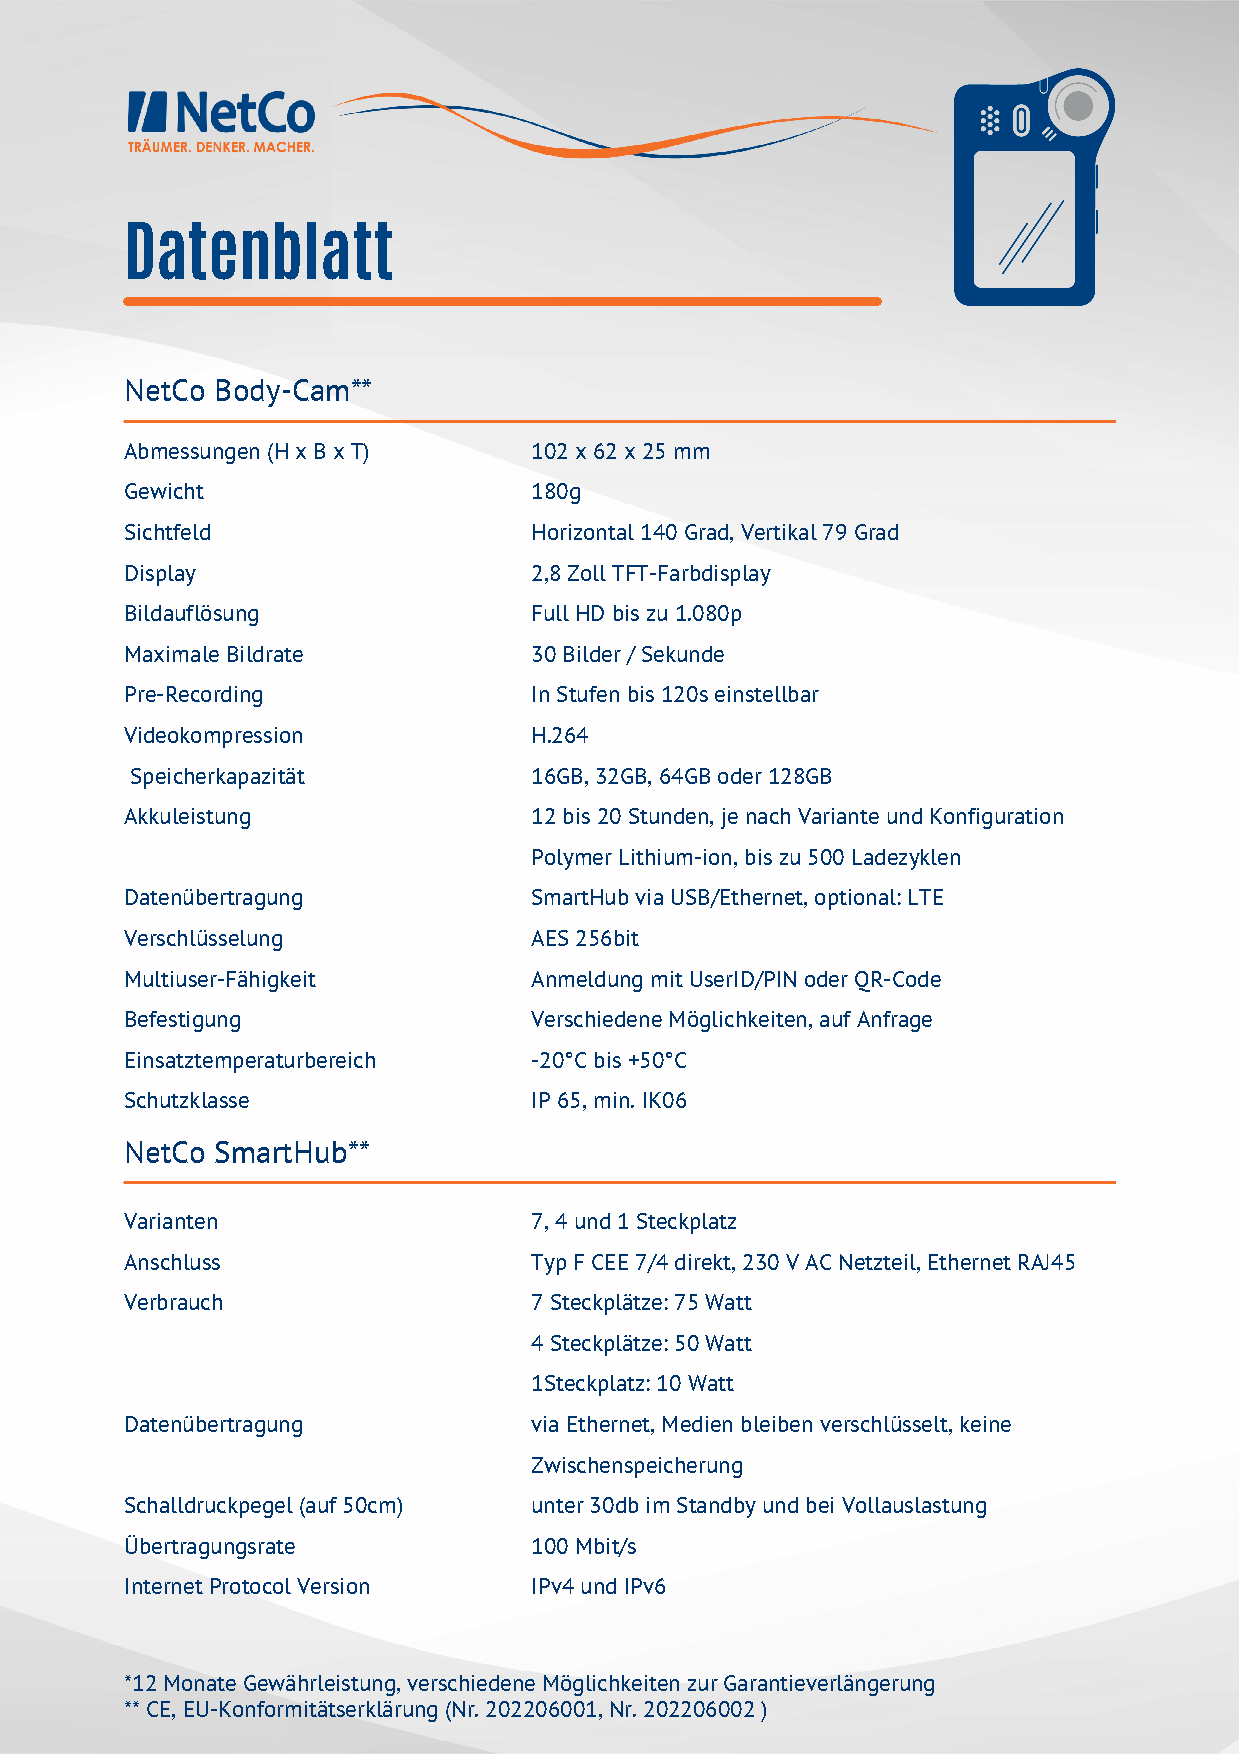
\includegraphics[page=1,width=\textwidth,height=.9\textheight,keepaspectratio]{../sources/Datenblatt_Bodycam.pdf}

\section{Testprotokoll}

\subsection*{Testfall 1: Verbindung herstellen}

\textbf{Beschreibung:}\\
Dieser Testfall überprüft, ob der Client erfolgreich eine Verbindung zum Server aufbauen kann. Der Client sendet eine Verbindungsanfrage an den Server und wartet auf einen erfolgreichen Handshake. Wenn die Verbindung erfolgreich hergestellt wurde, sendet der Client eine Initialnachricht an den Server der diesen über die Timeoutzeit informiert.

\textbf{Voraussetzungen:}
\begin{itemize}
    \item Der Server ist gestartet und lauscht auf Port 8080.
    \item Der Client kann den Server über seine URL erreichen.
\end{itemize}

\textbf{Schritte:}
\begin{enumerate}
    \item Der Client wird mit den Parameter Server-URL und Port 8080 gestartet.
    \item Der Client sendet eine Verbindungsanfrage an den Server.
    \item Der Server antwortet mit einem Handshake-Antwortpaket, das die erfolgreiche\\ Handshake-Bestätigung der Websocket-Verbindung signalisiert.
    \item Nach erfolgreichem Handshake sendet der Client eine Protokoll-Nachricht mit dem Typ \glqq initialMessage\grqq{} und der Timeoutzeit als Daten.
\end{enumerate}

\textbf{Erwartetes Ergebnis:}\\
Die Websocket-Verbindung zwischen Client und Server ist hergestellt und beide Seiten haben die gleiche Timeoutzeit.

\textbf{Ergebnis:}\\



\subsection*{Testfall 2: Heartbeat-Nachrichten senden}

\textbf{Beschreibung:}\\
Dieser Testfall überprüft, ob der Client und der Server in der Lage sind, erfolgreich Heartbeat-Nachrichten auszutauschen. Der Server sendet eine Nachricht an den Client und wartet auf eine Antwort. Wenn der Client die Nachricht empfängt, sendet er eine Antwort zurück. Beide Seiten setzten beim Empfangen einer Nachricht ihren Timer für Verbindungsverlust zurück.

\textbf{Voraussetzungen:}
\begin{itemize}
    \item Der Client ist mit dem Server verbunden.
    \item Der Server ist gestartet und lauscht auf Port 8080.
\end{itemize}

\textbf{Schritte:}
\begin{enumerate}
    \item Der Server sendet eine Heartbeat-Nachricht an den Client.
    \item Der Client empfängt die Nachricht und detektiert sie als Heartbeat.
    \item Der Client setzt seinen Timer zurück und schickt einen Heartbeat zurück an den Server.
    \item Der Server empfängt die Nachricht und detektiert sie als Heartbeat.
    \item Der Server setzt seinen Timer zurück.
\end{enumerate}

\textbf{Erwartetes Ergebnis:}\\
Der Heartbeat wurde erfolgreich zwischen beiden Seiten ausgetauscht und der Timer für Verbindungsverlust wurde zurückgesetzt.

\textbf{Ergebnis:}\\



\subsection*{Testfall 3: Verbindung wiederherstellen (erfolgreich)}

\textbf{Beschreibung:}\\
Dieser Testfall überprüft, ob der Client in der Lage ist, eine Verbindung zum Server wiederherzustellen, nachdem die Verbindung unterbrochen wurde. Der Client versucht, die Verbindung wiederherzustellen, nachdem die Verbindung unterbrochen wurde, und wartet auf eine Bestätigungsnachricht vom Server. Wenn die Verbindung erfolgreich wiederhergestellt wurde, können Nachrichten zwischen Client und Server ausgetauscht werden.

\textbf{Voraussetzungen:}
\begin{itemize}
    \item Der Client ist mit dem Server verbunden.
    \item Der Server ist gestartet und lauscht auf Port 8080.
\end{itemize}

\textbf{Schritte:}
\begin{enumerate}
    \item Die Verbindung zwischen Client und Server wird unterbrochen.
    \item Der Client stellt durch das Ausbleiben von Heartbeats fest, dass die Verbindung unterbrochen ist.
    \item Der Client versucht die Verbindung zum Server wieder herzustellen.
    \item Der Server antwortet mit einem Handshake-Antwortpaket, das die erfolgreiche\\ Handshake-Bestätigung der Websocket-Verbindung signalisiert.
    \item Beide Seiten tauschen Heartbeat-Nachrichten aus.
\end{enumerate}

\textbf{Erwartetes Ergebnis:}\\
Die Websocket-Verbindung zwischen Client und Server wird erfolgreich wiederhergestellt.

\textbf{Ergebnis:}\\



\subsection*{Testfall 4: Verbindung wiederherstellen (nicht erfolgreich)}

\textbf{Beschreibung:}\\
Dieser Testfall überprüft, ob der Client in der Lage ist, eine Verbindung zum Server wiederherzustellen, nachdem die Verbindung unterbrochen wurde. Der Client versucht, die Verbindung wiederherzustellen, nachdem die Verbindung unterbrochen wurde, und wartet auf eine Bestätigungsnachricht vom Server. Die Verbindung kann nicht erfolgreich in einer bestimmten Zeit wiederhergestellt werden und es kommt zum Alarmfall.

\textbf{Voraussetzungen:}
\begin{itemize}
    \item Der Client ist mit dem Server verbunden.
    \item Der Server ist gestartet und lauscht auf Port 8080.
\end{itemize}

\textbf{Schritte:}
\begin{enumerate}
    \item Die Verbindung zwischen Client und Server wird unterbrochen.
    \item Der Client stellt durch das Ausbleiben von Heartbeats fest, dass die Verbindung unterbrochen ist.
    \item Der Client versucht die Verbindung zum Server wieder herzustellen.
    \item Der Server antwortet nicht und die Verbindung bleibt unterbrochen.
    \item Beide Seiten geben nach einer bestimmten Zeit aus das die Verbindung unterbrochen ist und eine dauerhafte Überwachung nicht sichergestellt werden kann.
\end{enumerate}

\textbf{Erwartetes Ergebnis:}\\
Die Websocket-Verbindung zwischen Client und Server wird nicht erfolgreich wiederhergestellt. Beide Seiten teilen diesen Alarmfall über die Programmausgabe mit.

\textbf{Ergebnis:}\\



\end{document}